% !TeX spellcheck = de_DE

\chapter{Bildmodifusion}
\label{chap:fusion}

Nachdem im vorherigen Kapitel auf die Methode der Dilatation zur Verbesserung des erstellten Tiefenbildes eingegangen wurde, wird in diesem Kapitel der Vorgang der Kalibrierung beschrieben.
Dabei werden zuerst Problematiken der einzelnen Kameras beschrieben, um ein Verständnis für die auszugleichenden Schwächen zu schaffen.
Danach werden die betrachteten Fusionsmöglichkeiten und der Grund für ihr Verwerfen genannt, sowie die letztendlich gewählte Fusionsart beschrieben.

\section{Vor- und Nachteile der Kameras}
Um eine qualitative Fusion zu erreichen, muss ein Verständnis für die Stärken und Schwächen der jeweilig verwendeten Systeme vorhanden sein.
Im folgenden werden die für relevant erachteten Einschränkungen aufgelistet.

\subsection{Wärmebildkamera}
%\subsubsection{Wärmebildkamera}
\begin{center}
	\begin{tabular}{| p{7.5cm} | p{7.5cm} |}
		\hline
		Vorteile & Nachteile \\ \hline
		
		\begin{itemize}
			\item Kann Temperaturunterschiede darstellen
			\item Zeichnet sehr gute Konturen bei geringen Temperaturunterschieden
			\item Große Reichweite
			\item Ermöglicht Sicht durch diverse Materialien
		\end{itemize} & \begin{itemize}
			\item Wärmereflexion an vielen Materialien
			\item Schlechte Bildqualität bei nahezu nicht vorhandenem Temperaturunterschied
			\item \enquote{Wärmeflecken} an Orten, wo zuvor ein warmes Objekt war
			\item Geringere Auflösung / Kleinerer Blickwinkel
		\end{itemize} \\ 
		\hline
	\end{tabular}
\end{center}

\subsection{Tiefenbildkamera}
%\subsubsection{Tiefenbildkamera}
\begin{center}
	\begin{tabular}{| p{7.5cm} | p{7.5cm} |}
		\hline
		Vorteile & Nachteile \\ \hline
		
		\begin{itemize}
			\item Gute Darstellung von Konturen größerer Objekte
			\item Größere Auflösung / Größerer Blickwinkel
		\end{itemize} & \begin{itemize}
			\item Eingeschränkte Reichweite (\ca 0,5m - 7,5m)
			\item Flimmerndes Bild
			\item Teilweise werden kurze Distanzen nicht gut dargestellt
			\item Einige Materialien reflektieren
			\item Reflexion bei gewissem Haltungswinkel
			\item Einzelne Objektdetails schwerer zu erkennen
		\end{itemize} \\ 
		\hline
	\end{tabular}
\end{center}

\section{Explorierte Fusionsmöglichkeiten}
In diesem Abschnitt werden die genauer betrachteten Fusionsmöglichkeiten und der Grund für ihr verwerfen diskutiert.
Dabei sind in einigen der Abbildungen nicht die optimierten Bildarten integriert, da diese Möglichkeiten bereits früher verworfen wurden.

\subsection{Parallele Anzeige beider Modi}
Das Tiefenbild und das Wärmebild werden wie in \cref{fig:fusion_both} entweder nebeneinander oder übereinander angezeigt.
Dadurch könnten beide Bildmodi verlustfrei angezeigt werden, allerdings würden die Probleme nur begrenzt verringert werden.
\begin{figure}[H]
	\centering
	\begin{subfigure}[t]{0.25\textwidth}
		\centering
		\ifthenelse{\boolean{jpg}}{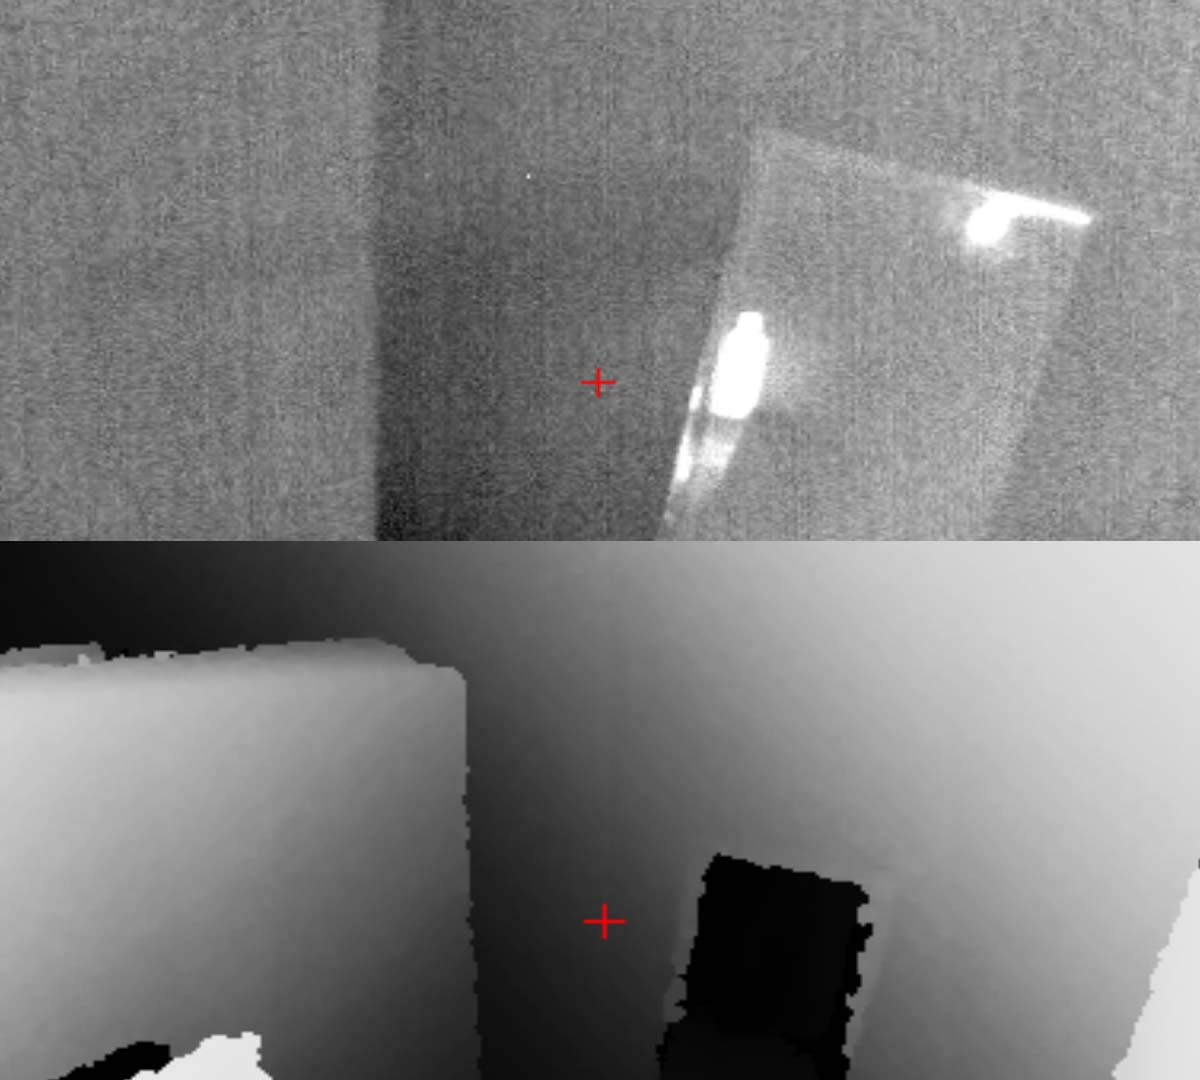
\includegraphics[width=\textwidth]{Fusion/over.jpg}}{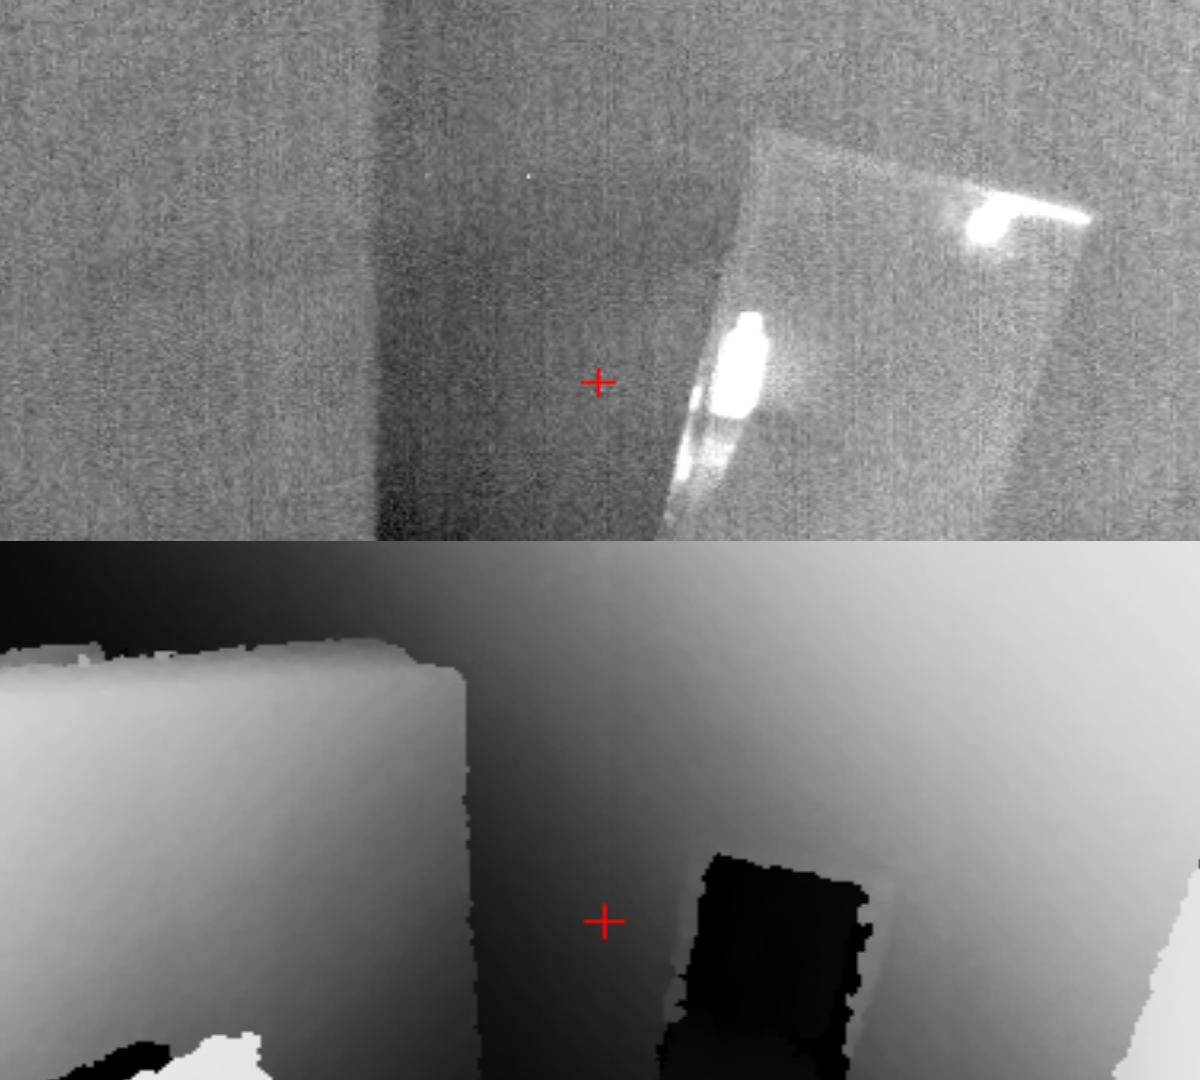
\includegraphics[width=\textwidth]{Fusion/over.png}}
		\caption{Anzeige beider Modi übereinander}
		\label{fig:fusion_both_over}
	\end{subfigure}
	~
	\begin{subfigure}[t]{0.65\textwidth}
		\centering
		\ifthenelse{\boolean{jpg}}{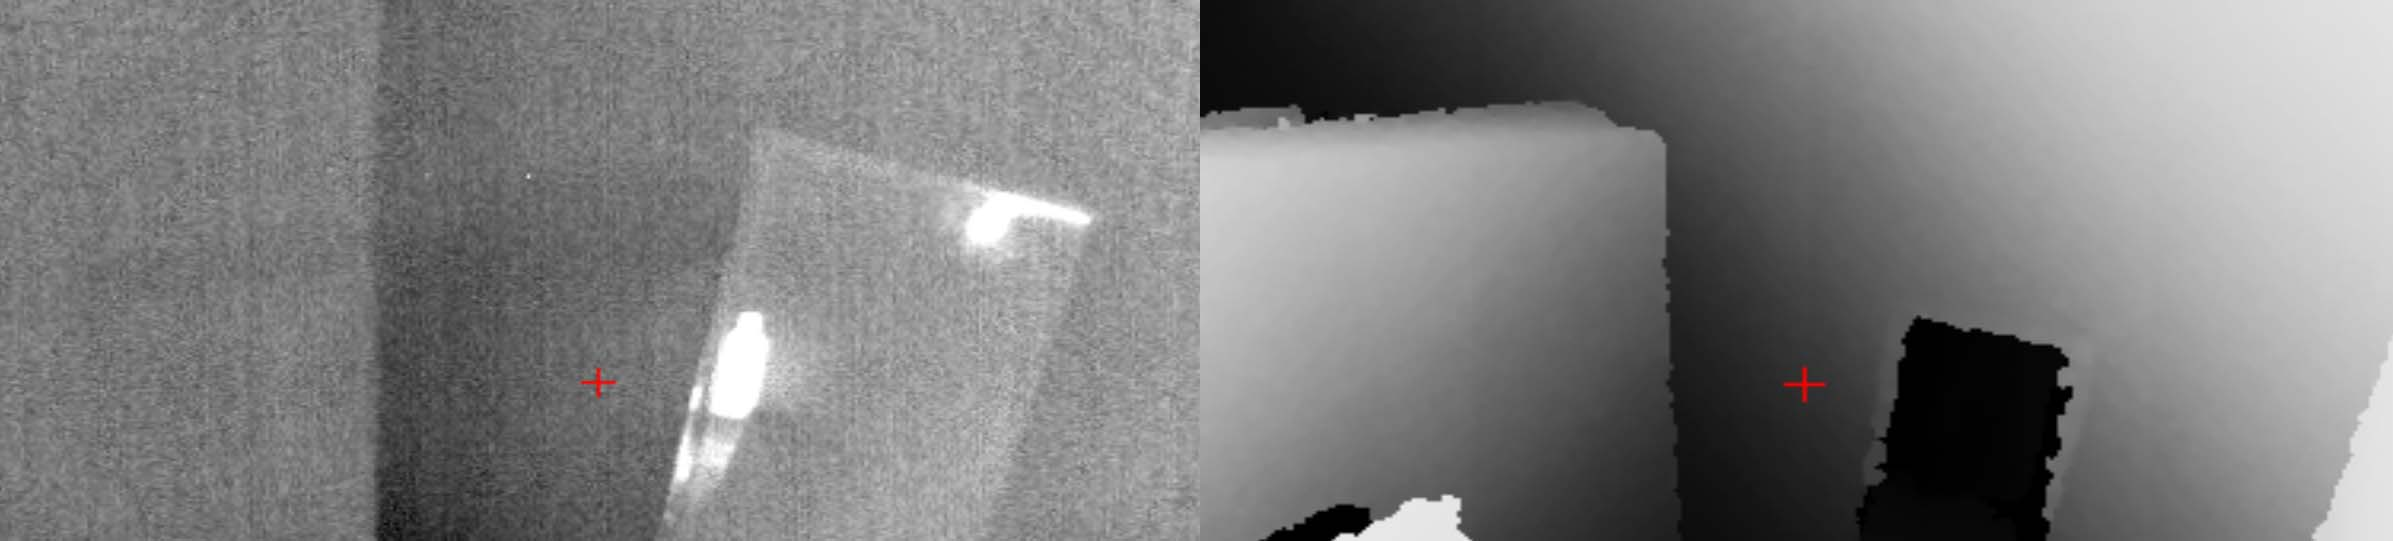
\includegraphics[width=\textwidth]{Fusion/besides.jpg}}{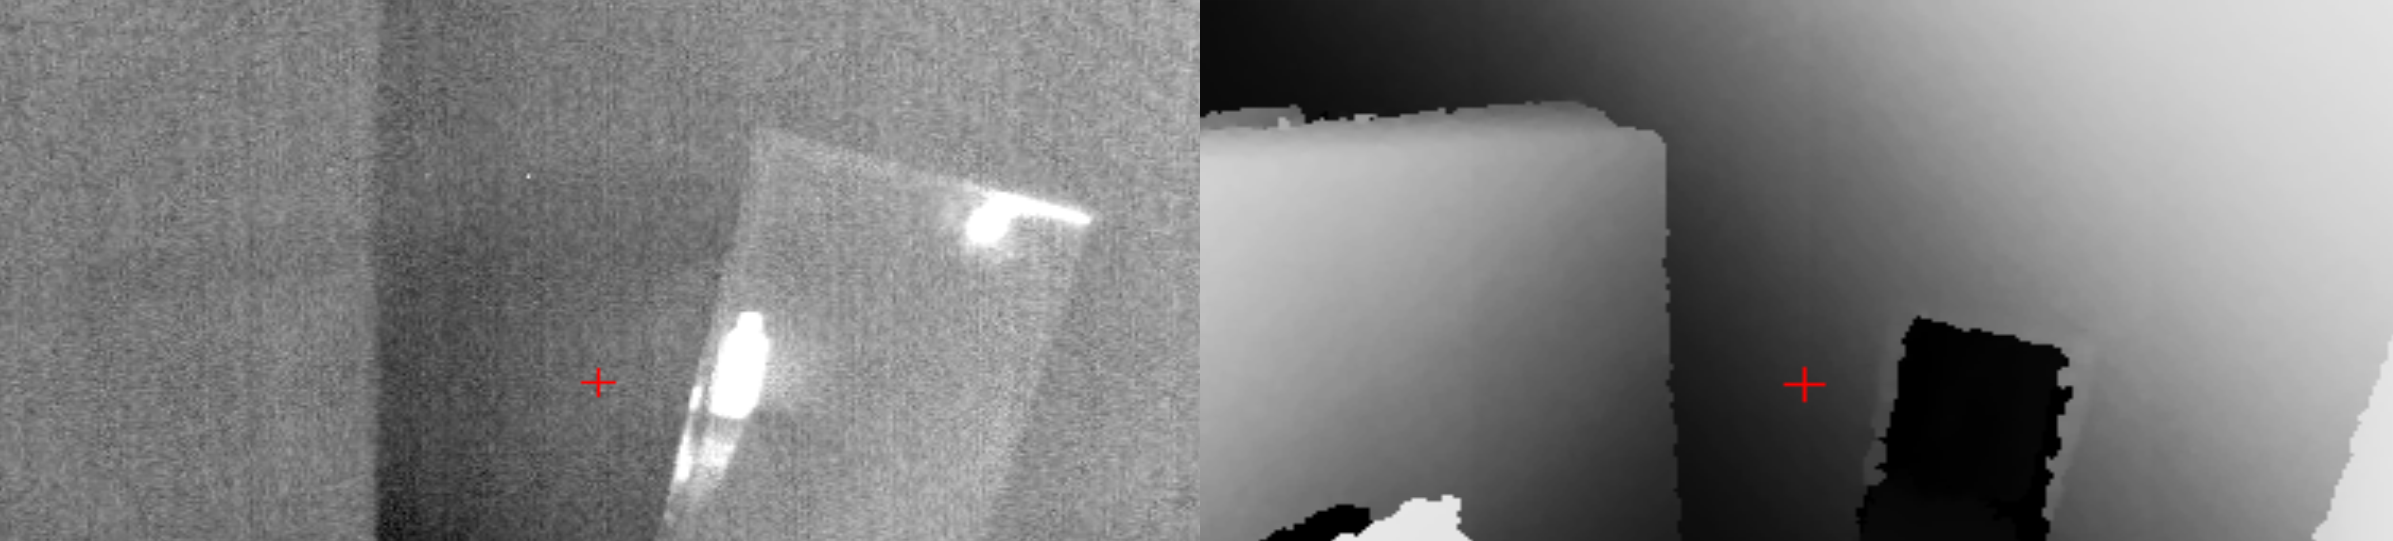
\includegraphics[width=\textwidth]{Fusion/besides.png}}
		\caption{Anzeige beider Modi nebeneinander}
		\label{fig:fusion_both_besides}
	\end{subfigure}
	\caption{Parallele Anzeige von beiden Kameramodi}
	\label{fig:fusion_both}
\end{figure}

Dieser Ansatz wurde verworfen, da dieser Ansatz keine wirkliche Fusion darstellt und bei internen Tests einige Teilnehmer noch Schwierigkeiten hatten, Objekte auf beiden Teilen zu lokalisieren.
Auch wirkte sich dieser Ansatz negativ auf das mobile Anzeigegerät, da die Anzeige bereits aus kurzer Entfernung für zu klein befunden wurde.

\subsection{Ersetzen des Tiefenbild mit Wärmebild}
\label{sec:fusion_overwrite}
\cref{fig:fusion_overwrite} zeigt, dass das Wärmebild über den Bildteil des normalen Tiefenbildes gelegt wird.
Problematisch hierbei ist, dass lediglich der Vorteil des größeren Bildausschnitts der Tiefenbildkamera genutzt wird.
Alle anderen Probleme bestehen weiterhin.
Zudem wurde, in Abstimmung mit den Projektbetreuern, entschieden, dass der unterschiedlich große Bildausschnitt, beider Kameras nicht beachtet und durch verkleinern der Auflösung der Tiefenbildkamera eliminiert wird, da dies durch ein anderes Objektiv der Wärmebild gelöst werden könnte.
\begin{figure}[H]
	\centering
	\ifthenelse{\boolean{jpg}}{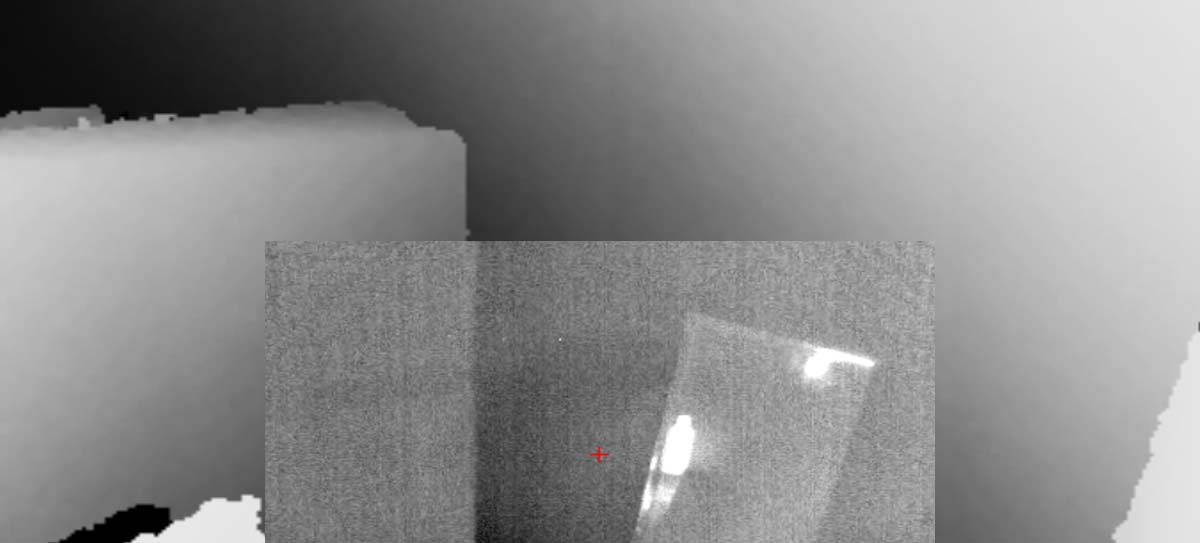
\includegraphics[width=0.9\textwidth]{Fusion/overwrite.jpg}}{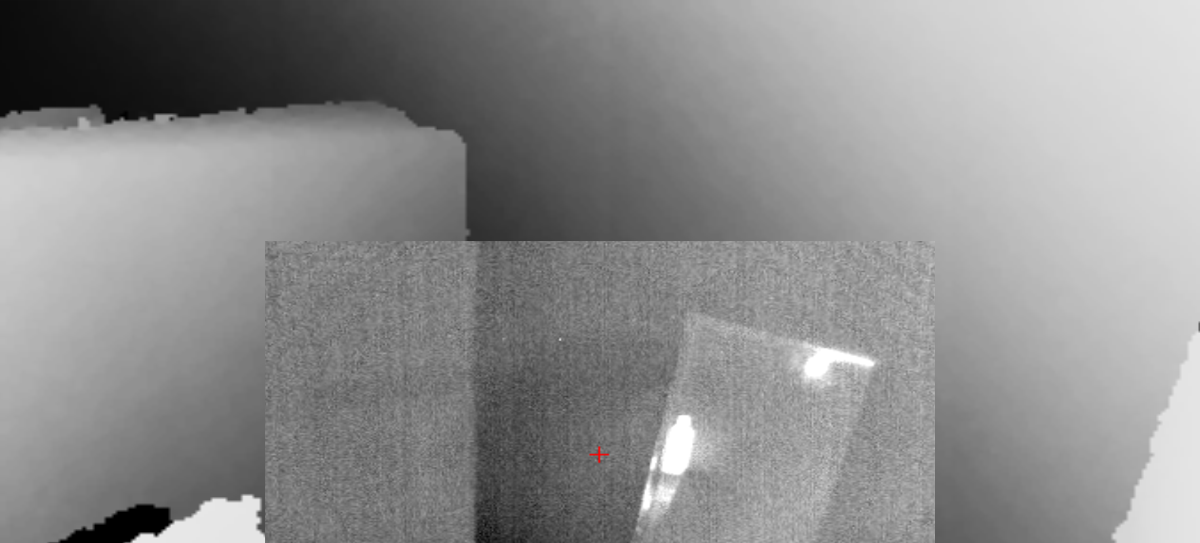
\includegraphics[width=0.9\textwidth]{Fusion/overwrite.png}}
	\caption{Ersetzung eines Teiles des Tiefenbildes mit Wärmebild}
	\label{fig:fusion_overwrite}
\end{figure}

\subsection{Semi-Transparenz des Wärmebilds über dem Tiefenbild}
Dieser Ansatz ist ähnlich der in \ref{sec:fusion_overwrite} beschriebenen Möglichkeit.
Der Unterschied besteht darin, dass anstelle das Tiefenbild mit dem Wärmebild zu ersetzen, das Wärmebild mit einem geringen Transparenzwert überlagert wird.
\begin{figure}[H]
	\centering
	\ifthenelse{\boolean{jpg}}{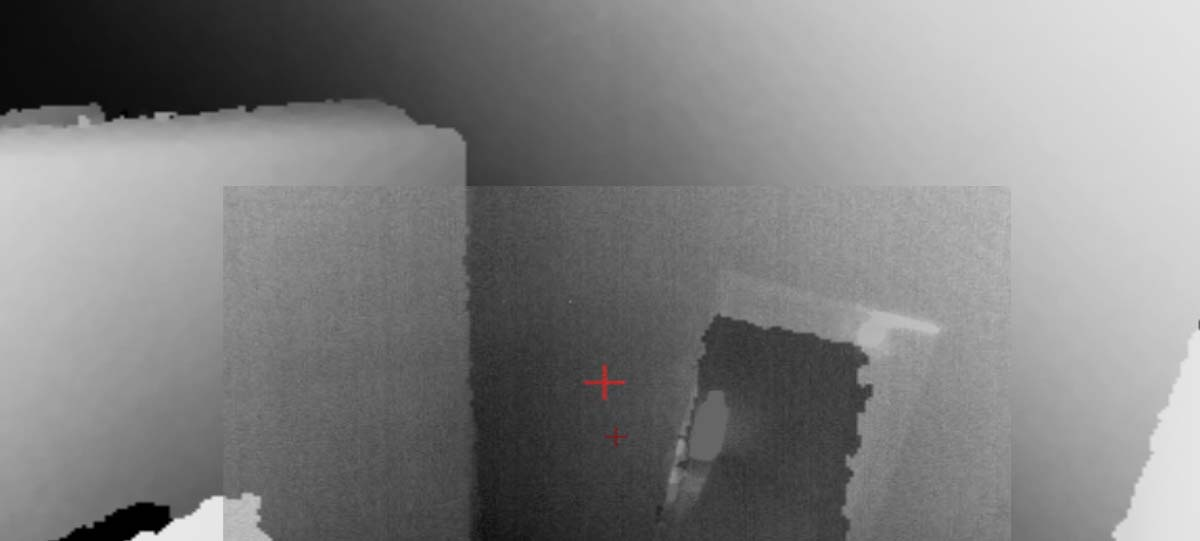
\includegraphics[width=\textwidth]{Fusion/transparenz.jpg}}{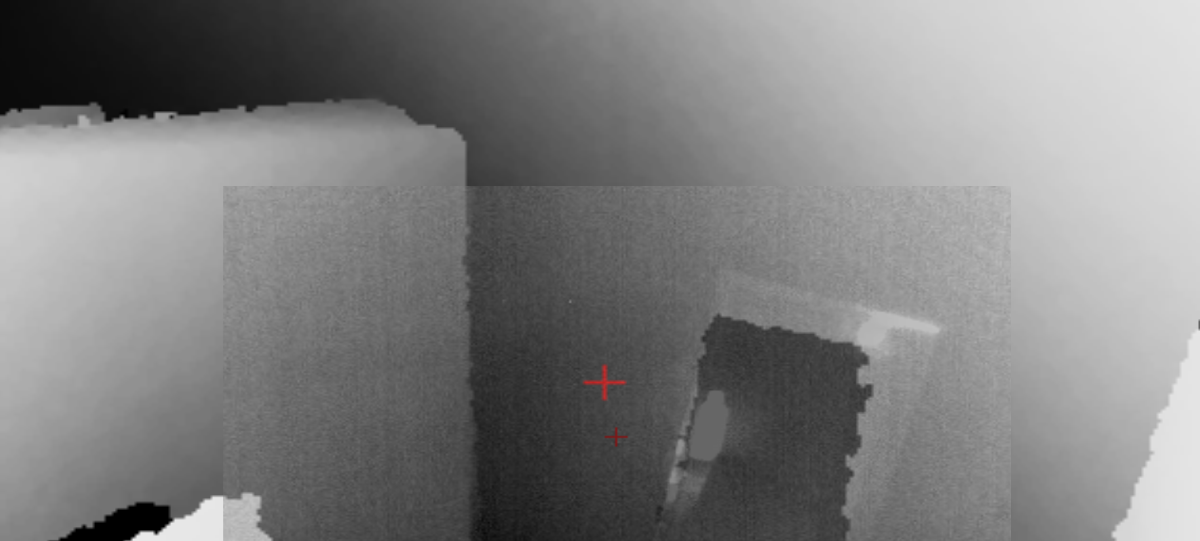
\includegraphics[width=\textwidth]{Fusion/transparenz.png}}
	\caption{Überlagerung eines Teiles des Tiefenbildes mit semitransparenten Wärmebild}
	\label{fig:fusion_transparenz}
\end{figure}

Gegen diesen Ansatz sprach, die oben beschriebene Entscheidung, das Tiefenbild auf die gleiche Größe, wie das Wärmebild zu regulieren.
Zudem sorgte, diese Überlagerung in bestimmten Kombinationen, wie heißer Gegenstand in mehr als 10m Entfernung, für ein unangenehmes Bild.
Letztendlich waren Reflexionen nicht besser zu erkennen.

\subsection{Konturen im Wärmebild nachzeichnen}
\label{sec:fusion_lines}
Diese Möglichkeit sieht das Nachzeichnen von Konturen im Wärmebild, mit den Informationen des Tiefenbildes vor.
\begin{figure}[H]
	\centering
	\begin{subfigure}[t]{0.45\textwidth}
		\centering
		\ifthenelse{\boolean{jpg}}{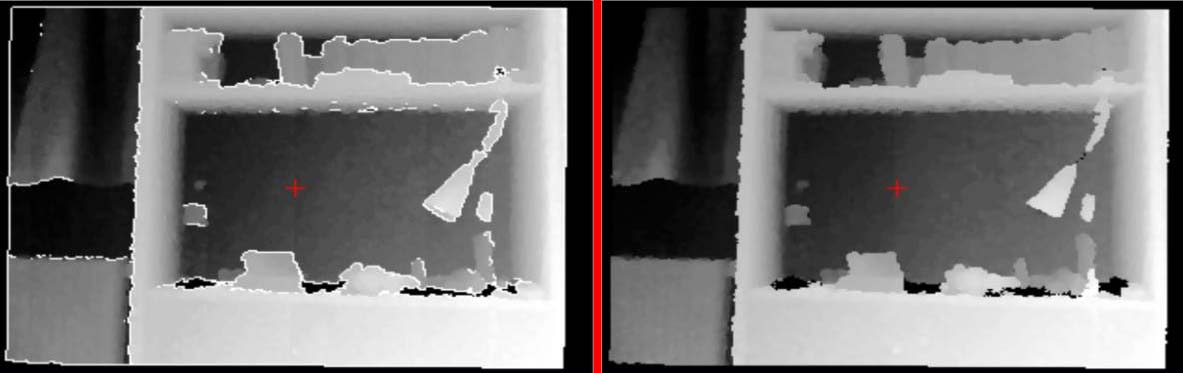
\includegraphics[width=\textwidth]{Fusion/lines3.jpg}}{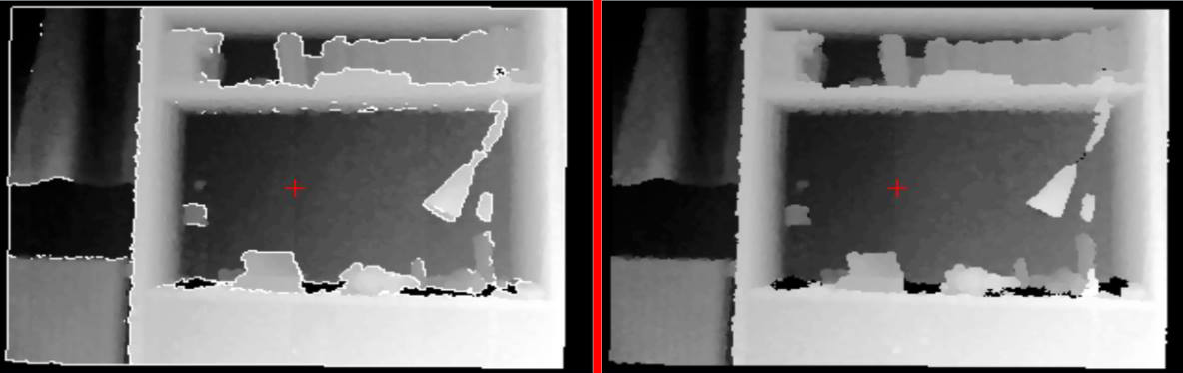
\includegraphics[width=\textwidth]{Fusion/lines3.png}}
		\caption{Sehr gute Konturennachzeichnung}
		\label{fig:fusion_lines3}
	\end{subfigure}
	~
	\begin{subfigure}[t]{0.45\textwidth}
		\centering
		\ifthenelse{\boolean{jpg}}{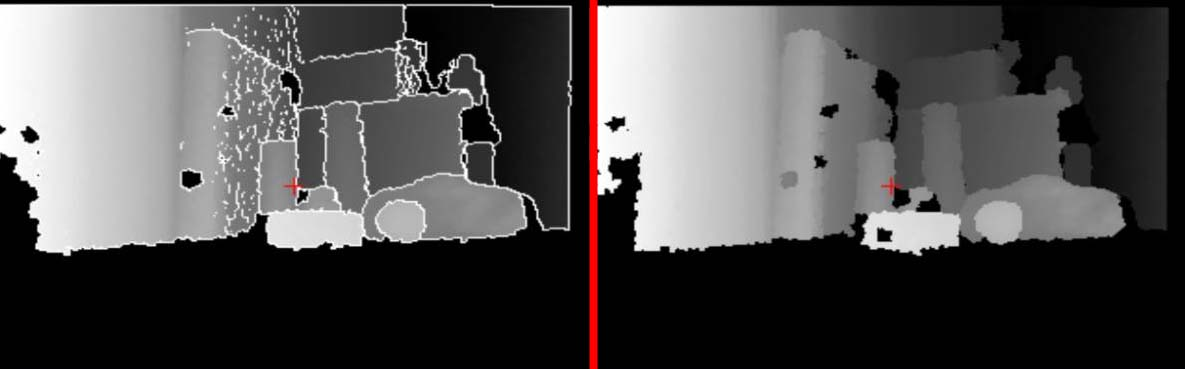
\includegraphics[width=\textwidth]{Fusion/lines1.jpg}}{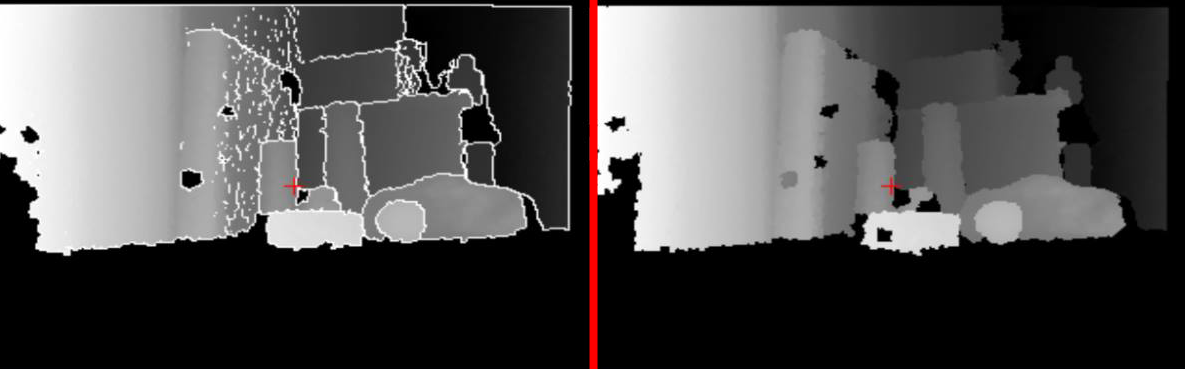
\includegraphics[width=\textwidth]{Fusion/lines1.png}}
		\caption{Gute Konturennachzeichnung}
		\label{fig:fusion_lines1}
	\end{subfigure}
	\caption{Konturenverbesserung mit Hilfe von Linien im Tiefenbild}
	\label{fig:fusion_lines_good}
\end{figure}
\begin{figure}[H]
	\centering
	\begin{subfigure}[t]{0.55\textwidth}
		\centering
		\ifthenelse{\boolean{jpg}}{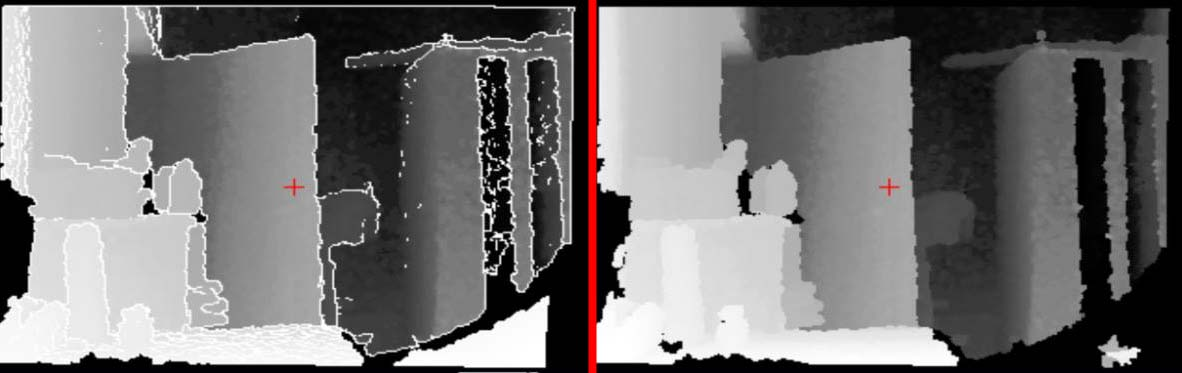
\includegraphics[width=\textwidth]{Fusion/lines2.jpg}}{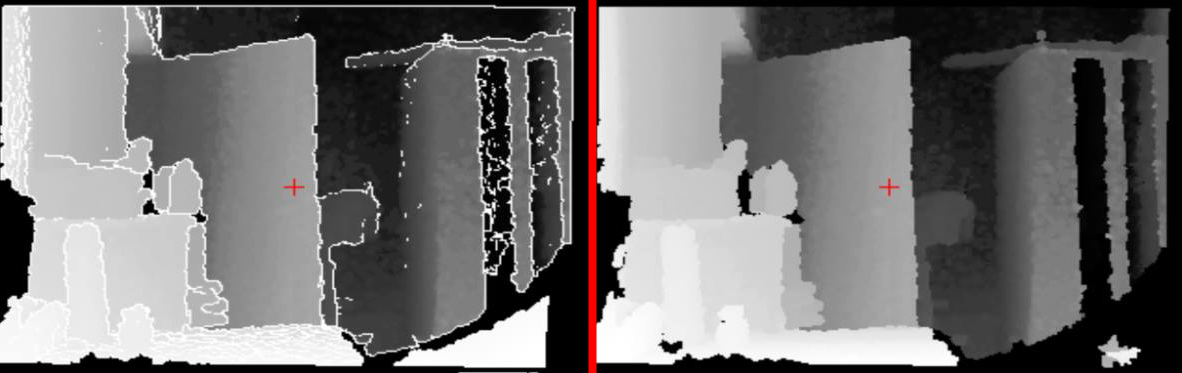
\includegraphics[width=\textwidth]{Fusion/lines2.png}}
		\caption{Konturennachzeichnung mit einigen Fehlern}
		\label{fig:fusion_lines2}
	\end{subfigure}
	~
	\begin{subfigure}[t]{0.35\textwidth}
		\centering
		\ifthenelse{\boolean{jpg}}{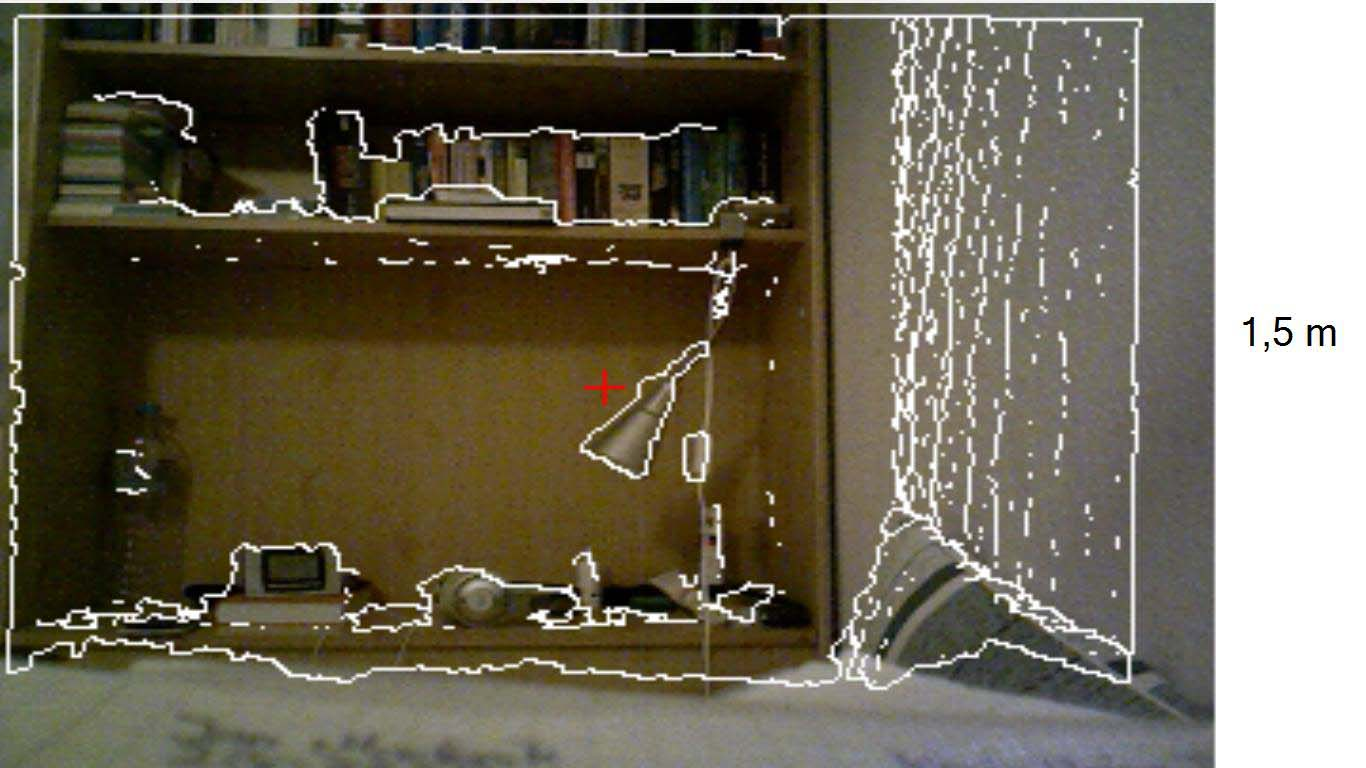
\includegraphics[width=\textwidth]{Fusion/lines.jpg}}{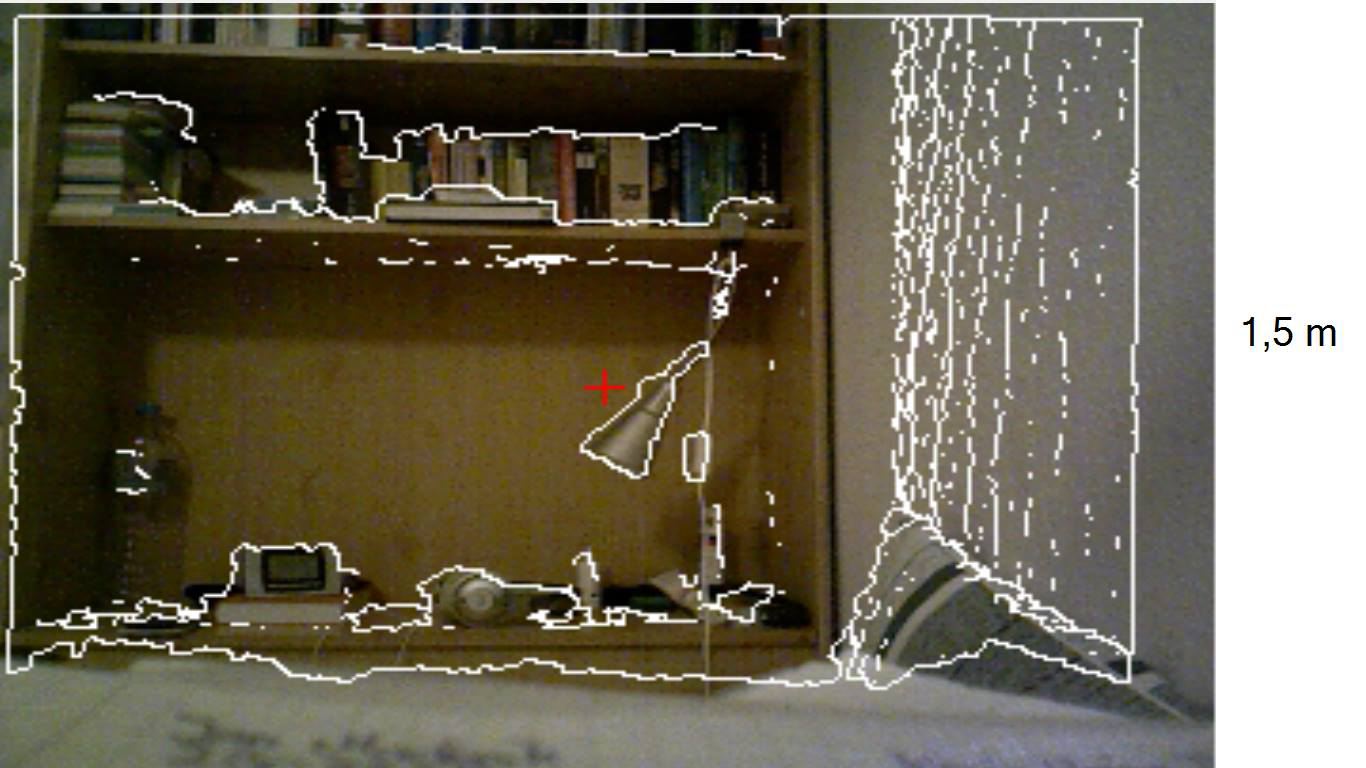
\includegraphics[width=\textwidth]{Fusion/lines.png}}
		\caption{Konturennachzeichnung mit vielen Fehlern im RGB-Bild}
		\label{fig:fusion_lines}
	\end{subfigure}
	\caption{Konturenverbesserung mit Hilfe von Linien im Tiefenbild}
	\label{fig:fusion_lines_bad}
\end{figure}

Obwohl dieser Ansatz, wie in \cref{fig:fusion_lines_good} zu sehen, gute Ergebnisse im Tiefenbild produziert, sorgt er in anderen Bildmodi, wie in \cref{fig:fusion_lines_bad}, zu der fehlerhaften Anzeige von vielen zusätzlichen Konturen.
Zusätzlich zu dem häufig fehlerhaften Ergebnis, kommt ein Performanceverlust, welcher selten Verzögerungen im Bild oder Standbilder zur Folge hatte.
Da dies in einer sicherheitskritischen Real-Time Anwendung nicht tragbar ist, wurde dieser Ansatz verworfen.

\subsection{Temperaturunterschiede im Tiefenbild nachzeichnen}
\label{sec:fusion_post-render}
Bei dieser Möglichkeit wird nur das Tiefenbild gezeichnet.
Falls die Wärmebildkamera nun einen Gegenstand erfasst, welcher eine andere Temperatur hat, wird dieser Bereich im Tiefenbild mit den Informationen der Wärmebild überschrieben.
Diskutierte Metriken waren eine lokale Temperaturabweichung um einem zu bestimmenden Prozentsatz von der Durchschnittstemperatur oder eine lokale Temperaturabweichung von der unmittelbaren Umgebung.
\cref{fig:fusion_post-render} zeigt, das gewünschte Ergebnis, allerdings wurde in der Realität häufig die Umgebung des zu zeichnenden Objekts mit übernommen.
Dies führte zu dem Verlust der Möglichkeit, Reflexionen zuverlässig zu erkennen.
Außerdem war eine zuverlässige Kalibrierung hier nur schwer zu erreichen.
Zusätzlich hatte diese Methode eine spürbar negative Wirkung auf die Performance.
\begin{figure}[H]
	\centering
	\ifthenelse{\boolean{jpg}}{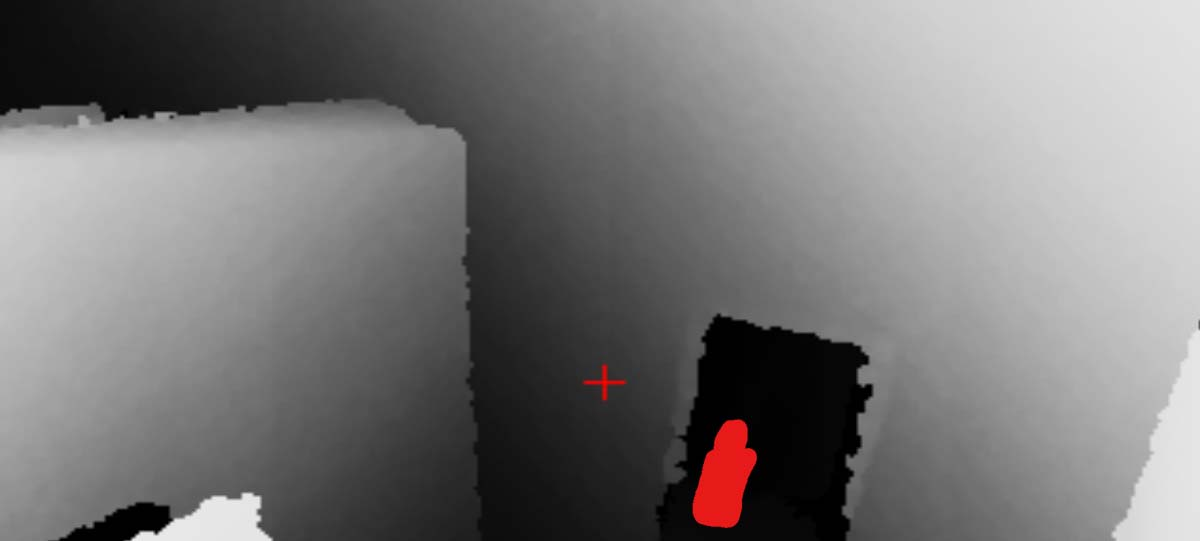
\includegraphics[width=\textwidth]{Fusion/post-render.jpg}}{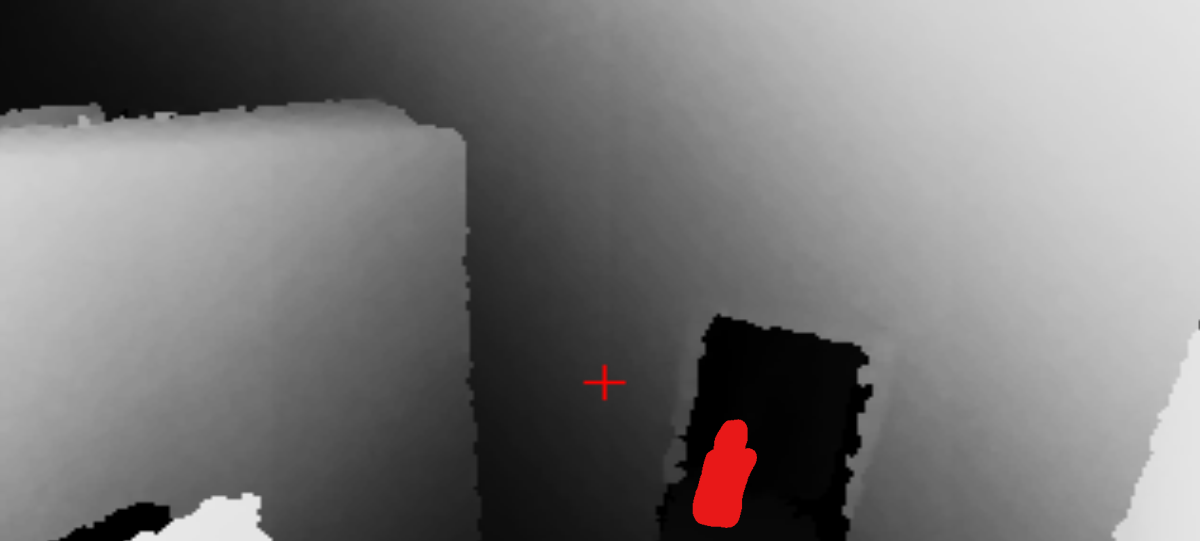
\includegraphics[width=\textwidth]{Fusion/post-render.png}}
	\caption{Nachträgliches Überschreiben des Tiefenbildes mit ausgewählten Wärmebildinformation}
	\label{fig:fusion_post-render}
\end{figure}

\subsection{Dynamischer Bildmodiwechsel}
Dieser Ansatz war als Mischung aus \cref{sec:fusion_lines} und \cref{sec:fusion_post-render} geplant.
Dabei würde hauptsächlich das Tiefenbild angezeigt werden, allerdings mit den nachgezeichneten Linien, für eine bessere Konturendarstellung.
In \cref{fig:fusion_dyn_depth} ist schematisch das identifizieren von Objekten anhand dieser Linien dargestellt.
Wenn nun ein bestimmtes Kriterium getroffen wird, wird automatisch auf das Tiefenbild gewechselt.
Sobald das Kriterium nicht mehr eingehalten wird, wird wieder das Tiefenbild angezeigt.
Angedachte Kriterien waren unter anderem die Metriken aus \cref{sec:fusion_post-render}, aber auch Eigenschaften wie ein Prozentsatz an nicht vorhandenen Tiefenbildinformationen, welcher nicht überschritten werden darf oder ein festgelegter Temperaturunterschied der einen automatischen Wechsel auslöst.
Ebenso wie das automatische Wechseln, falls ein warmes Objekt in der Nähe des Bildmittelpunktes erkannt wird.
\begin{figure}[H]
	\centering
	\begin{subfigure}[t]{0.45\textwidth}
		\centering
		\ifthenelse{\boolean{jpg}}{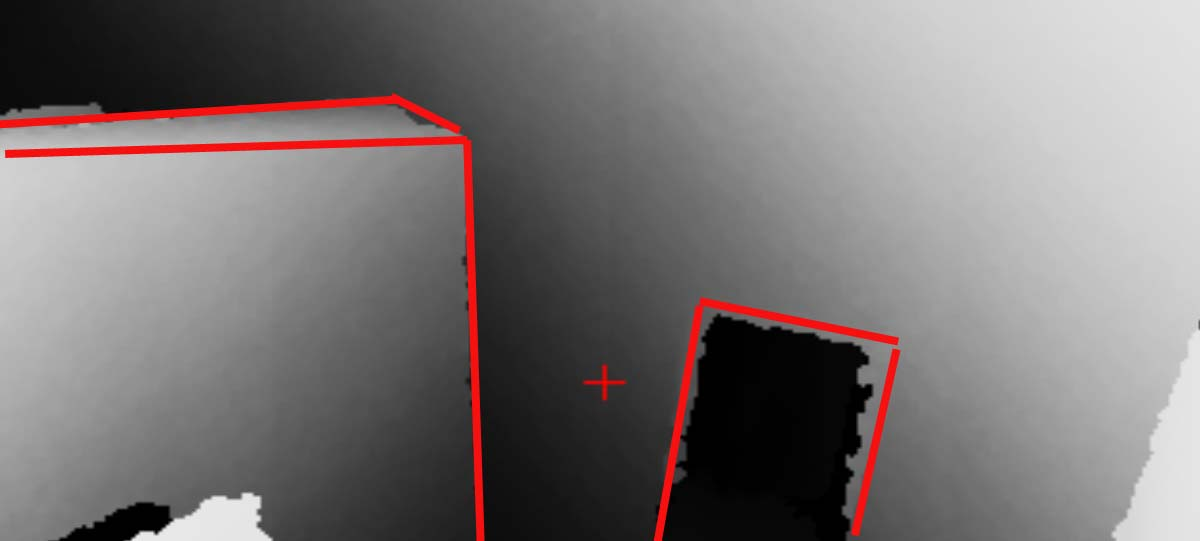
\includegraphics[width=\textwidth]{Fusion/dyn_depth.jpg}}{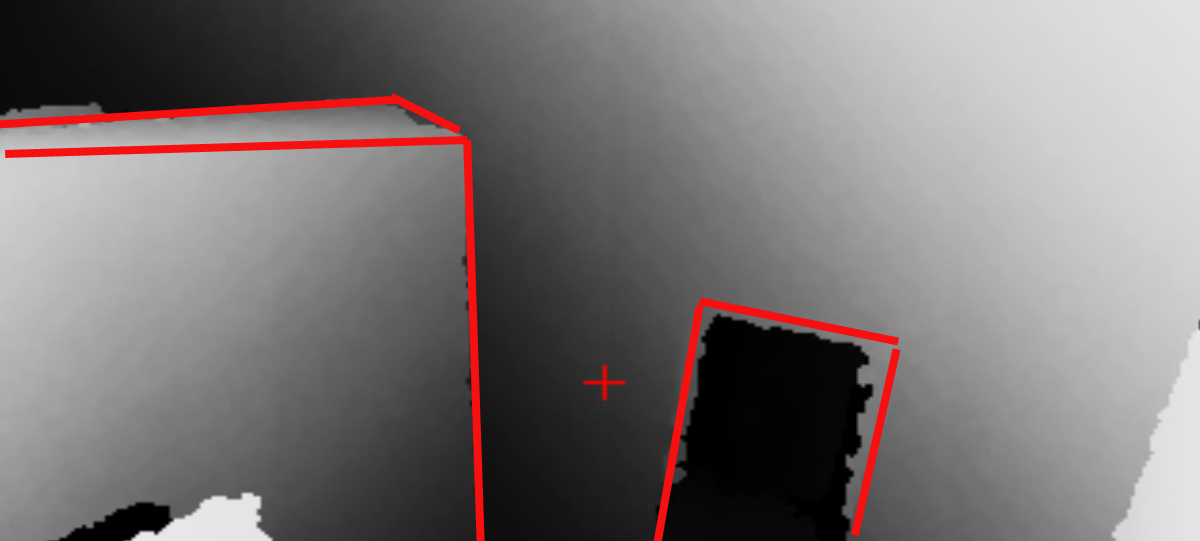
\includegraphics[width=\textwidth]{Fusion/dyn_depth.png}}
		\caption{Objekterkennung im Tiefenbild mittels Konturennachzeichnung}
		\label{fig:fusion_dyn_depth}
	\end{subfigure}
	~
	\begin{subfigure}[t]{0.45\textwidth}
		\centering
		\ifthenelse{\boolean{jpg}}{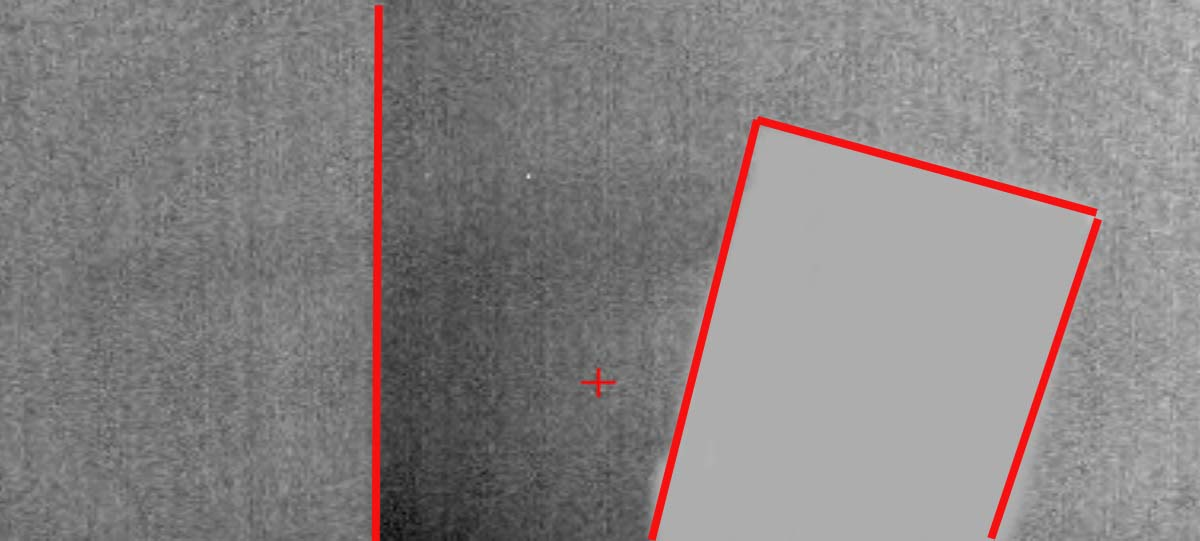
\includegraphics[width=\textwidth]{Fusion/dyn_heat.jpg}}{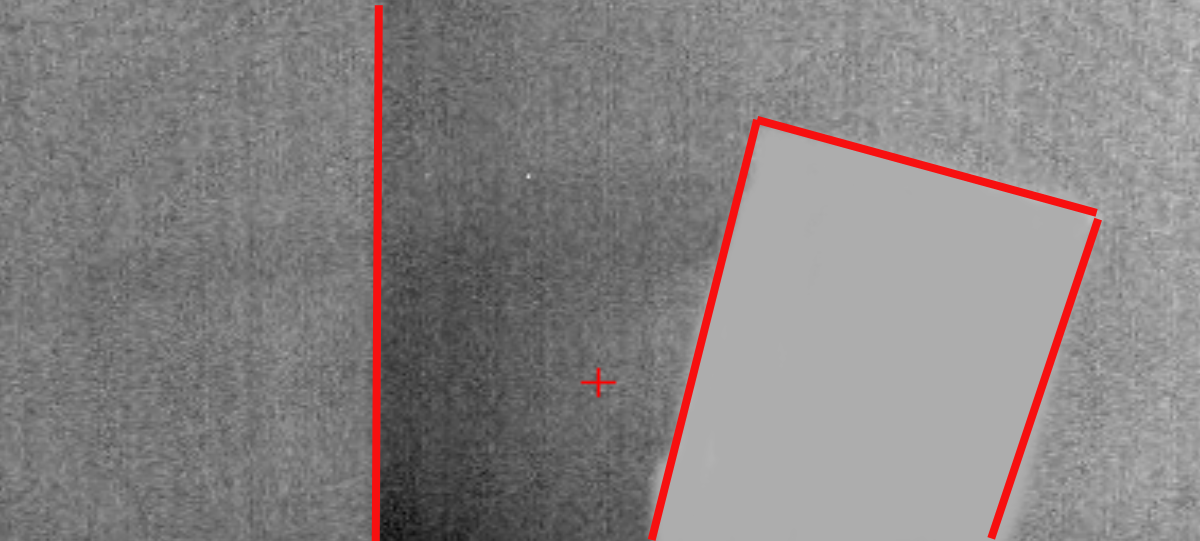
\includegraphics[width=\textwidth]{Fusion/dyn_heat.png}}
		\caption{Entfernung von Reflexionen mittels kontextbezogener Temperatur}
		\label{fig:fusion_dyn_heat}
	\end{subfigure}
	\caption{Dynamischer Kamerawechsel}
	\label{fig:fusion_dyn}
\end{figure}

Das Wärmebild wird nun mit den aus dem Tiefenbild erhaltenen Informationen, über die enthaltenen Objekte, verbessert.
Dabei wird die wärmste und kälteste Temperatur in diesem Objekt gesucht.
Wird dabei ein Unterschied festgestellt, wird das komplette Objekt mit der Durchschnittstemperatur dieses Objekts belegt.
Durch diese Maßnahme könnten nahezu alle Reflexionen und \enquote{fehlerhafte} Wärmeflecke eliminiert werden.
\cref{fig:fusion_dyn_heat} zeigt wie ein solches Wärmebild aussehen könnte.


Problematisch an diesem Ansatz ist, zum einen der enorme Performanceverlust, der mit der mehrmaligen Überprüfung jedes gelieferten Bildes einhergeht.
Selbst eine Reduktion der Bildüberprüfungsfrequenz führte zu keiner akzeptablen Laufzeit.
Zum weiterhin würden auch warme Objekte, wie \zB ein Induktionskochfeld mit nur einer aktivierten Platte, ihre korrekte Information verlieren.
Auch ist es nicht mehr möglich, durch dünne Wände hindurch Wärmestrahlung anzuzeigen.
Ein weiteres Problem ist, die in \cref{sec:fusion_lines} angesprochene Fehleranfälligkeit der Konturennachzeichnung.
Ohne einen guten und zuverlässigen \enquote{Linienalgorithmus}, kann die Objekterkennung nicht verlässlich funktionieren.

\section{Gewählte Fusionsmöglichkeit}
Der Fusionsansatz, welcher letztendlich umgesetzt wurde, vervierfacht die ursprüngliche Auflösung.
Dies passiert, indem das Tiefenbild als Ausgangsbild verwendet wird und nun zwischen jeden Tiefenbildpixel der entsprechende Wärmebildpixel gelegt wird.
Darauf wird zwischen jede \enquote{normale} Spalte, eine weitere Spalte eingefügt, in welcher Tiefenbildpixel zwischen den entsprechenden Wärmebildpixel eingefügt werden.
\cref{fig:fusion_pixel} stellt das schematisch entstehende Gitter dar.
Dabei ist zu erkennen, dass jeder Pixel beider Kameras nun zweifach im Gitter enthalten ist.
\begin{figure}[t]
	\centering
	\ifthenelse{\boolean{jpg}}{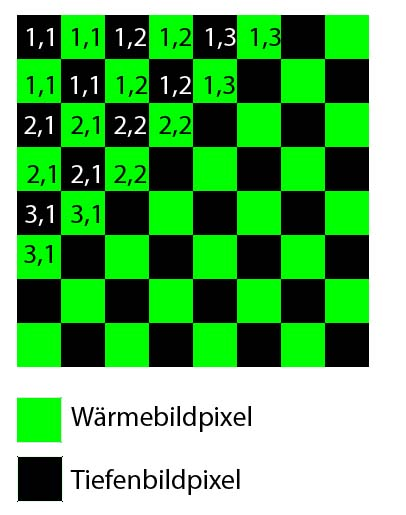
\includegraphics[scale=3.5]{Fusion/pixel.jpg}}{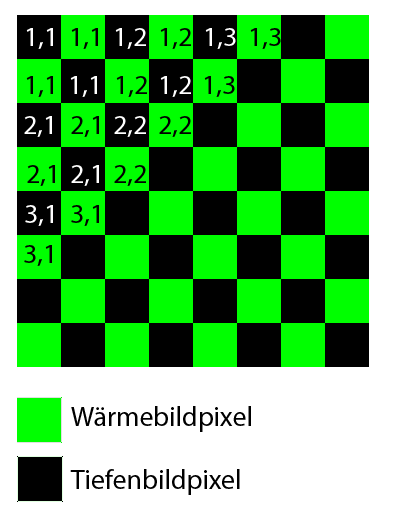
\includegraphics[scale=3.5]{Fusion/pixel.png}}
	\caption{Position der alten Pixel im entstandenes Fusionsgitter}
	\label{fig:fusion_pixel}
\end{figure}

Durch diesen Ansatz, bekommt das Wärmebild eine weitere Schnitt.
Nahe Objekte schimmern nun heller, entfernte Gegenstände haben dagegen eine dunklere Farbe.
Auch Wärmereflexionen sind besser zu erkennen, da die überlagerte Schicht um das angezeigte Objekt, die gleiche \enquote{Dicke} hat.
Diese fehlende Konturverstärkung um Objekte, ist damit als Symptom einer Reflexion oder glatten Fläche zu deuten.

In \cref{fig:fusion_fus} kann man erkennen, dass das Wärmebild relativ originalgetreu dargestellt wird.
Das Tiefenbild sorgt auf kurze Distanzen für eine helle \enquote{Schattierung}, wogegen auf größere Distanzen das Bild dunkler wird.
Dies erzeugt einen \enquote{3D-Effekt}, der für die räumliche Wahrnehmung vorteilhaft sein sollte.
\begin{figure}[H]
	\centering
	\begin{subfigure}[t]{0.45\textwidth}
		\centering
		\ifthenelse{\boolean{jpg}}{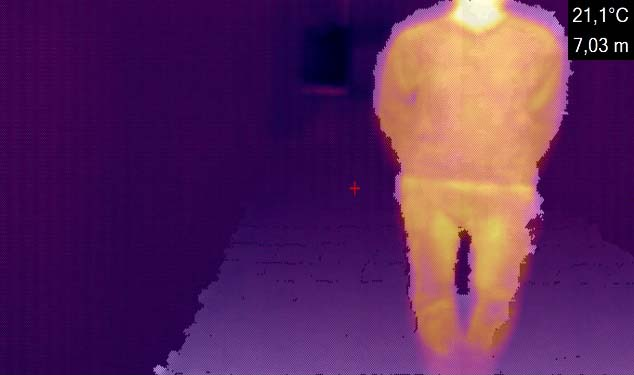
\includegraphics[width=\textwidth]{Fusion/fus1.jpg}}{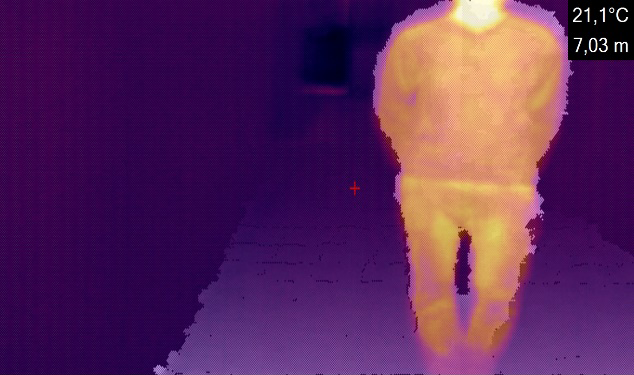
\includegraphics[width=\textwidth]{Fusion/fus1.png}}
		\caption{Objekterkennung im Tiefenbild mittels Konturennachzeichnung}
		\label{fig:fusion_fus1}
	\end{subfigure}
	~
	\begin{subfigure}[t]{0.45\textwidth}
		\centering
		\ifthenelse{\boolean{jpg}}{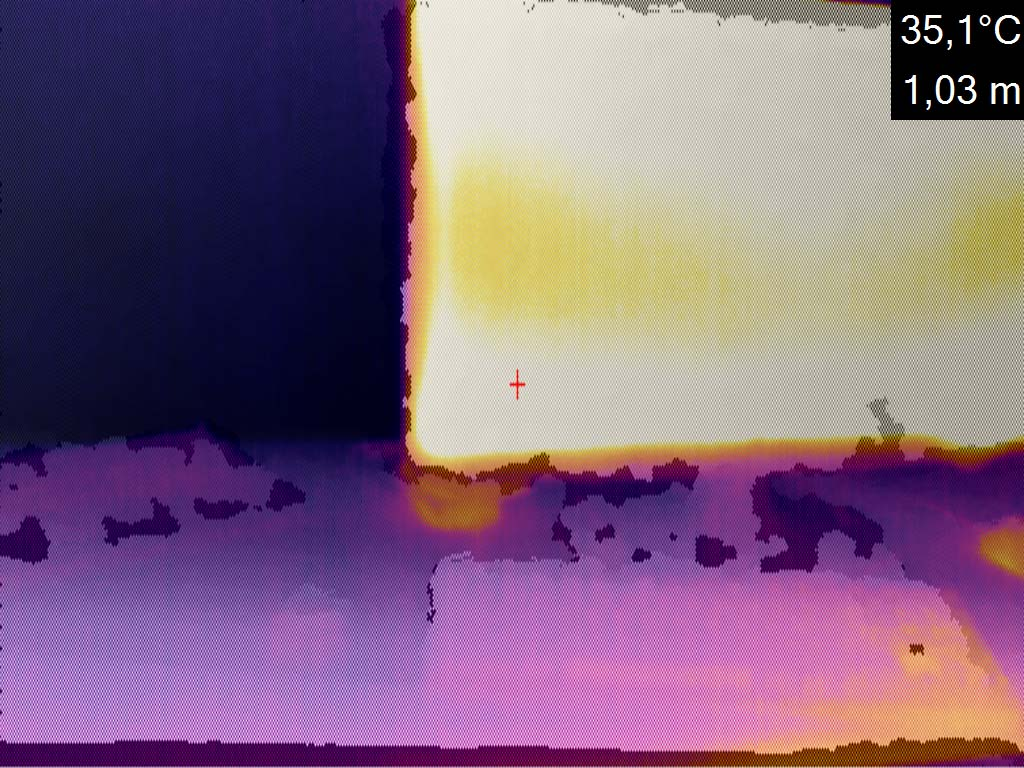
\includegraphics[width=\textwidth]{Fusion/fus2.jpg}}{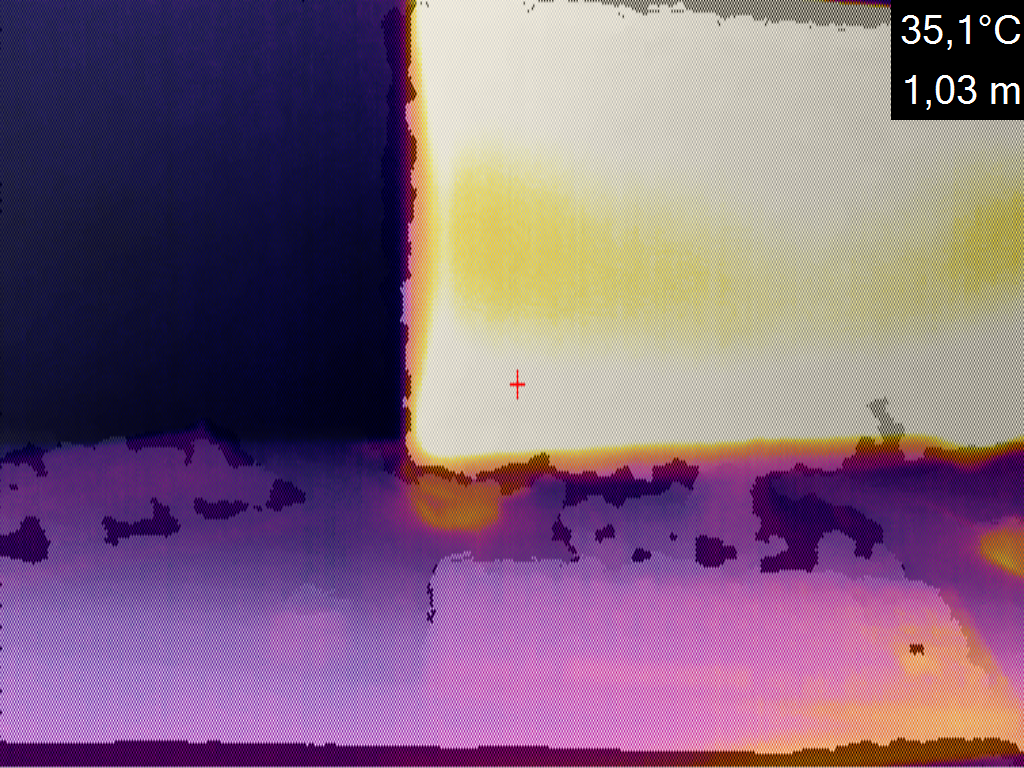
\includegraphics[width=\textwidth]{Fusion/fus2.png}}
		\caption{Entfernung von Reflexionen mittels kontextbezogener Temperatur}
		\label{fig:fusion_fus2}
	\end{subfigure}
	\caption{Implementierer Fusionsansatz}
	\label{fig:fusion_fus}
\end{figure}